\section{Observations}

\begin{enumerate}
    \item{\textbf{Ripple Up Counter}}

\begin{table}[H]
    \centering
    \begin{tabular}{|c|c|c|c|c|c|}\hline
          & \multicolumn{4}{c|}{Binary Count} &         \\ \hline
    Input & $Q_3$  & $Q_2$  & $Q_1$  & $Q_0$  & Decimal \\
    Pulse & $2^3$  & $2^2$  & $2^1$  & $2^0$  & Count   \\ \hline
    0     & 0      & 0      & 0      & 0     & 0       \\
    1     & 0      & 0      & 0      & 1     & 1       \\
    2     & 0      & 0      & 1      & 0     & 2       \\
    3     & 0      & 0      & 1      & 1     & 3       \\
    4     & 0      & 1      & 0      & 0     & 4       \\
    5     & 0      & 1      & 0      & 1     & 5       \\
    6     & 0      & 1      & 1      & 0     & 6       \\
    7     & 0      & 1      & 1      & 1     & 7       \\
    8     & 1      & 0      & 0      & 0     & 8       \\
    9     & 1      & 0      & 0      & 1     & 9       \\
    10    & 1      & 0      & 1      & 0     & 10       \\
    11    & 1      & 0      & 1      & 1     & 11       \\
    12    & 1      & 1      & 0      & 0     & 12       \\
    13    & 1      & 1      & 0      & 1     & 13       \\
    14    & 1      & 1      & 1      & 0     & 14       \\
    15    & 1      & 1      & 1      & 1     & 15      \\
    16    & 0      & 0      & 0      & 0     & 0 (RESET)    \\ \hline
    \end{tabular}
    \caption{Characterstic Table for a Ripple Up Counter Circuit (Refer Fig. \ref{up})}
\end{table}

\begin{figure}[H]
    \centering
    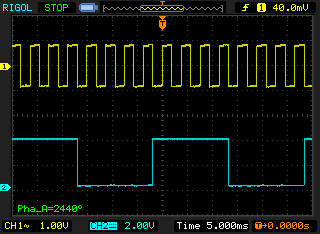
\includegraphics[width=.9\columnwidth]{images/oscilloscope.png}
    \caption{The oscilloscope output for the least (above) and the most significant bit (below), i.e. $Q_0$ and $Q_3$ in a 4-bit ripple up counter circuit. One can observe that the frequency of $Q_3$ is 1/4th that of $Q_0$}
\end{figure}



% \vspace{21pt}
\item{\textbf{MOD-12 Ripple Up Counter}}

\begin{table}[H]
    \centering
    \begin{tabular}{|c|c|c|c|c|c|}\hline
          & \multicolumn{4}{c|}{Binary Count} &         \\ \hline
    Input & $Q_3$  & $Q_2$  & $Q_1$  & $Q_0$  & Decimal \\
    Pulse & $2^3$  & $2^2$  & $2^1$  & $2^0$  & Count   \\ \hline
    0     & 0      & 0      & 0      & 0     & 0       \\
    1     & 0      & 0      & 0      & 1     & 1       \\
    2     & 0      & 0      & 1      & 0     & 2       \\
    3     & 0      & 0      & 1      & 1     & 3       \\
    4     & 0      & 1      & 0      & 0     & 4       \\
    5     & 0      & 1      & 0      & 1     & 5       \\
    6     & 0      & 1      & 1      & 0     & 6       \\
    7     & 0      & 1      & 1      & 1     & 7       \\
    8     & 1      & 0      & 0      & 0     & 8       \\
    9     & 1      & 0      & 0      & 1     & 9       \\
    10    & 1      & 0      & 1      & 0     & 10       \\
    11    & 1      & 0      & 1      & 1     & 11       \\
    12    & 0      & 0      & 0      & 0     & 0 (RESET)    \\ \hline
    \end{tabular}
    \caption{Characterstic Table for a MOD-12 Ripple Up Counter Circuit (Refer Fig. \ref{mod})}
\end{table}

\item{\textbf{Ring Counter}}

\begin{table}[H]
    \centering
    \begin{tabular}{|c|cccc|}
    \hline
    \multirow{2}{*}{\begin{tabular}[c]{@{}c@{}}Input\\ Pulses\end{tabular}} & \multicolumn{4}{c|}{\begin{tabular}[c]{@{}c@{}}Binary\\ States\end{tabular}}                 \\ \cline{2-5} 
                                                                                     & \multicolumn{1}{c|}{$Q_3$} & \multicolumn{1}{c|}{$Q_2$} & \multicolumn{1}{c|}{$Q_1$} & $Q_0$ \\ \hline
    0                                                                                & \multicolumn{1}{c|}{0}     & \multicolumn{1}{c|}{0}     & \multicolumn{1}{c|}{0}     & 1     \\ 
    1                                                                                & \multicolumn{1}{c|}{0}     & \multicolumn{1}{c|}{0}     & \multicolumn{1}{c|}{1}     & 0     \\ 
    2                                                                                & \multicolumn{1}{c|}{0}     & \multicolumn{1}{c|}{1}     & \multicolumn{1}{c|}{0}     & 0     \\ 
    3                                                                                & \multicolumn{1}{c|}{1}     & \multicolumn{1}{c|}{0}     & \multicolumn{1}{c|}{0}     & 0     \\ 
    4                                                                                & \multicolumn{1}{c|}{0}     & \multicolumn{1}{c|}{0}     & \multicolumn{1}{c|}{0}     & 1     \\ 
    5                                                                                & \multicolumn{1}{c|}{0}     & \multicolumn{1}{c|}{0}     & \multicolumn{1}{c|}{1}     & 0     \\ 
    6                                                                                & \multicolumn{1}{c|}{0}     & \multicolumn{1}{c|}{1}     & \multicolumn{1}{c|}{0}     & 0     \\ 
    7                                                                                & \multicolumn{1}{c|}{1}     & \multicolumn{1}{c|}{0}     & \multicolumn{1}{c|}{0}     & 0     \\ 
    8                                                                                & \multicolumn{1}{c|}{0}     & \multicolumn{1}{c|}{0}     & \multicolumn{1}{c|}{0}     & 1     \\ \hline
    \end{tabular}
    \caption{Characterstic Table for a Ring Counter Counter Circuit (Refer Fig. \ref{ring})}
\end{table}
\item{\textbf{Ripple Down Counter}}


\begin{table}[H]
    \centering
    \begin{tabular}{|c|c|c|c|c|c|}\hline
          & \multicolumn{4}{c|}{Binary Count} &         \\ \hline
    Input & $Q_3$  & $Q_2$  & $Q_1$  & $Q_0$  & Decimal \\
    Pulse & $2^3$  & $2^2$  & $2^1$  & $2^0$  & Count   \\ \hline
    0     & 0      & 0      & 0      & 0     & 0       \\
    1    & 1      & 1      & 1      & 1     & 15      \\
    2    & 1      & 1      & 1      & 0     & 14       \\
    3    & 1      & 1      & 0      & 1     & 13       \\
    4    & 1      & 1      & 0      & 0     & 12       \\
    5    & 1      & 0      & 1      & 1     & 11       \\
    6    & 1      & 0      & 1      & 0     & 10       \\
    7     & 1      & 0      & 0      & 1     & 9       \\
    8     & 1      & 0      & 0      & 0     & 8       \\
    9     & 0      & 1      & 1      & 1     & 7       \\
    10     & 0      & 1      & 1      & 0     & 6       \\
    11     & 0      & 1      & 0      & 1     & 5       \\
    12     & 0      & 1      & 0      & 0     & 4       \\
    13     & 0      & 0      & 1      & 1     & 3       \\
    14     & 0      & 0      & 1      & 0     & 2       \\
    15     & 0      & 0      & 0      & 1     & 1       \\
    16    & 0      & 0      & 0      & 0     & 0 (RESET)    \\ \hline
    \end{tabular}
    \caption{Characterstic Table for a Ripple Down Counter Circuit (Refer Fig. \ref{down})}
\end{table}
\end{enumerate}
